% %
% \begin{figure}[t]
% 	\centering
% 	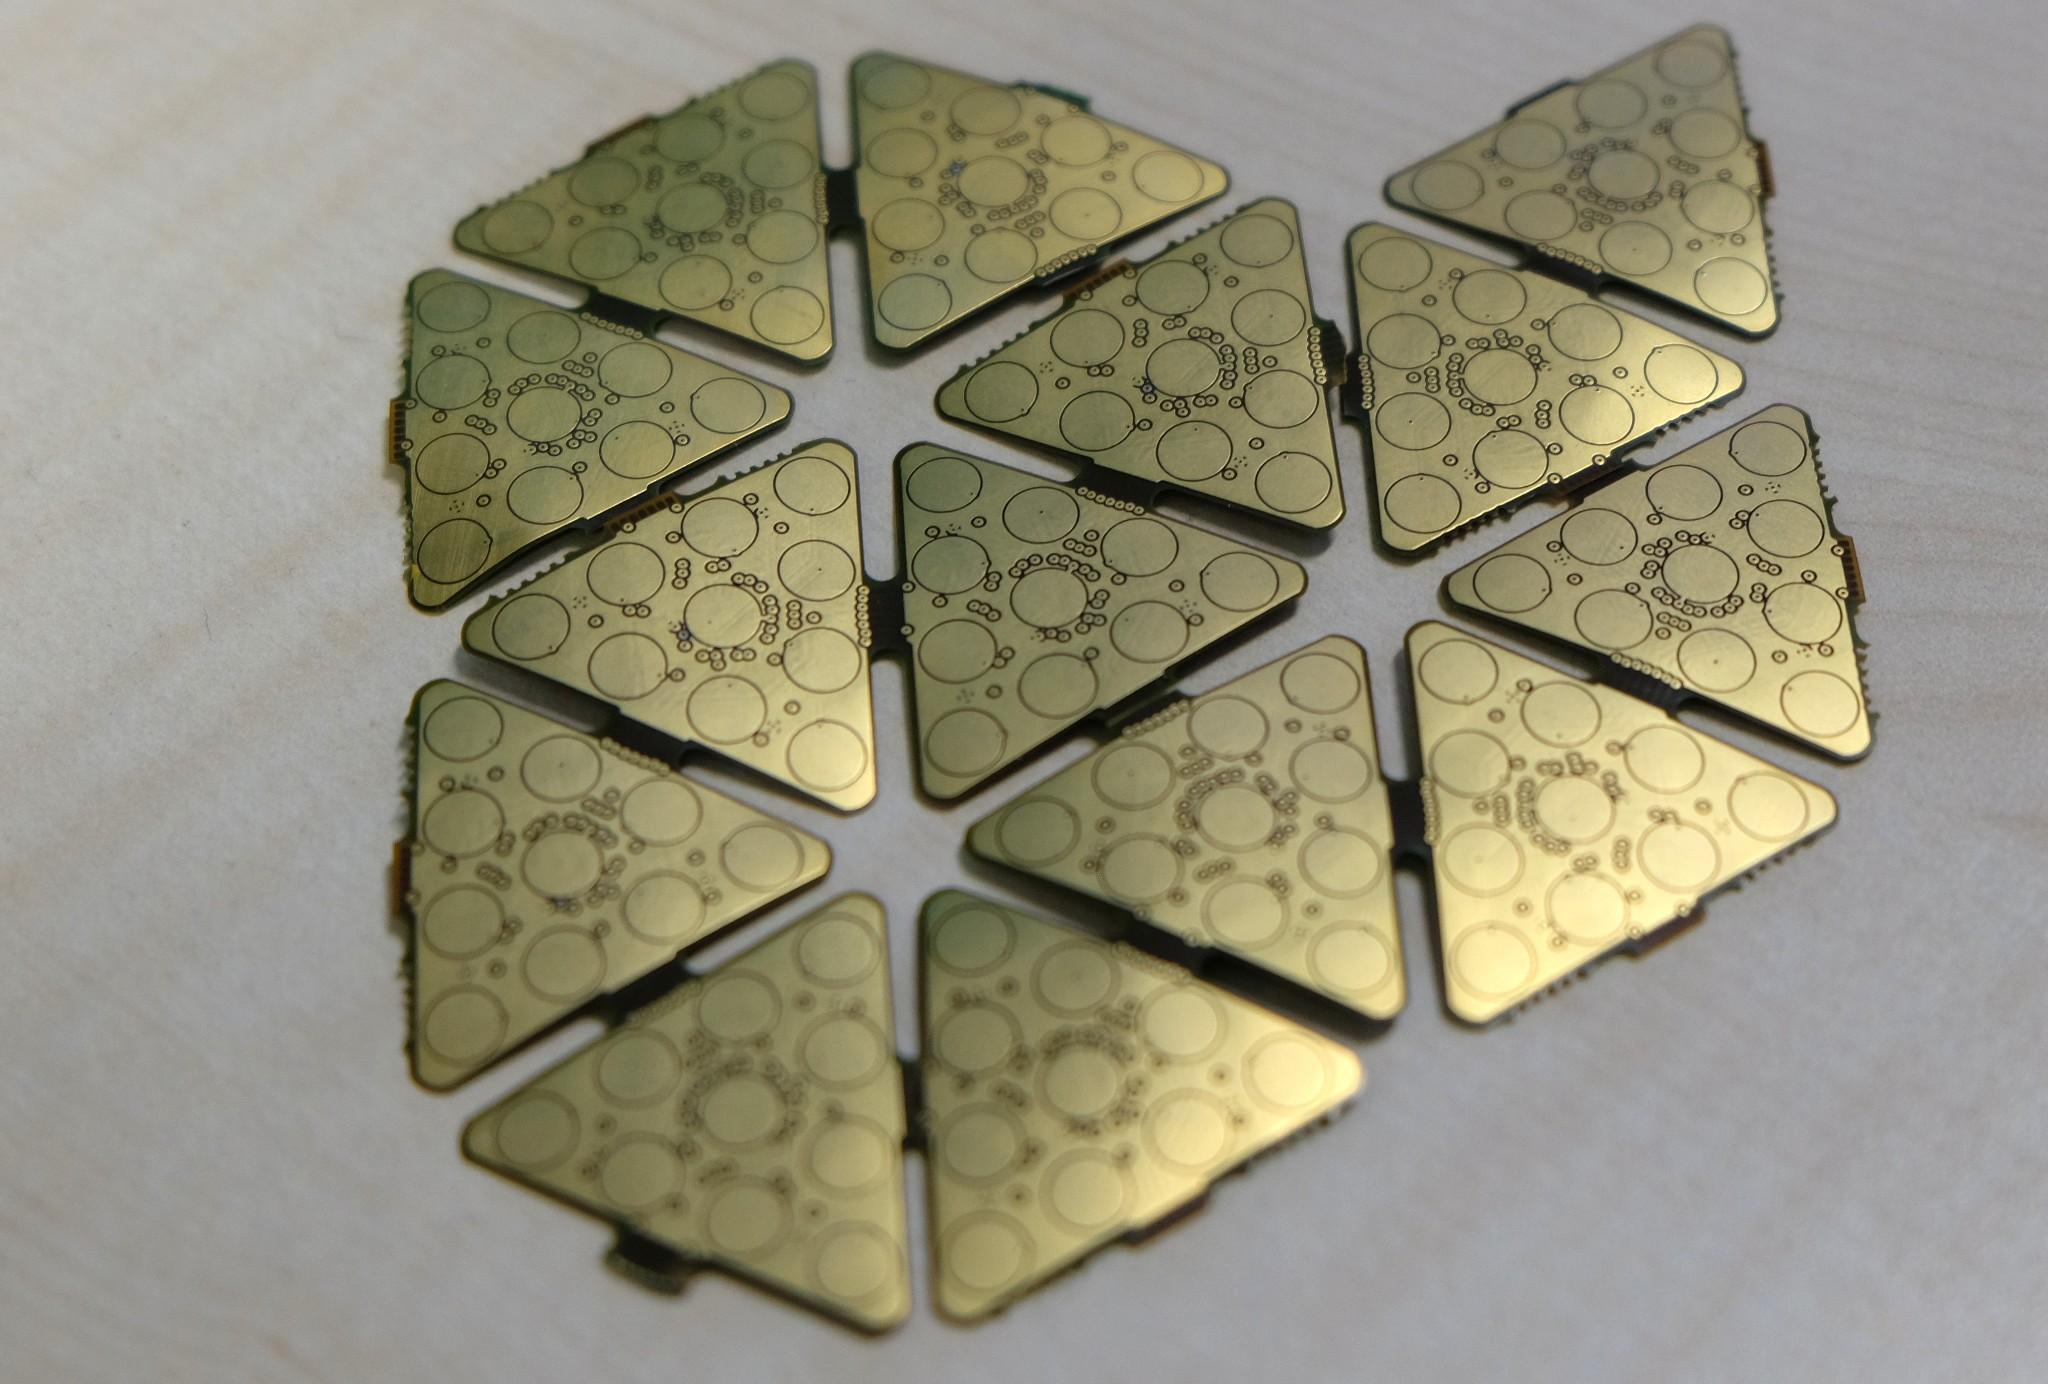
\includegraphics[width=.98\columnwidth]{fig/Skin1b}
% 	\caption{\robot{} Skin.}
% 	\label{fig:Fox_controller}
% \end{figure}
% %

%
% \begin{figure}[t]
% \resizebox{\hsize}{!}{
% 	\centering
% 	%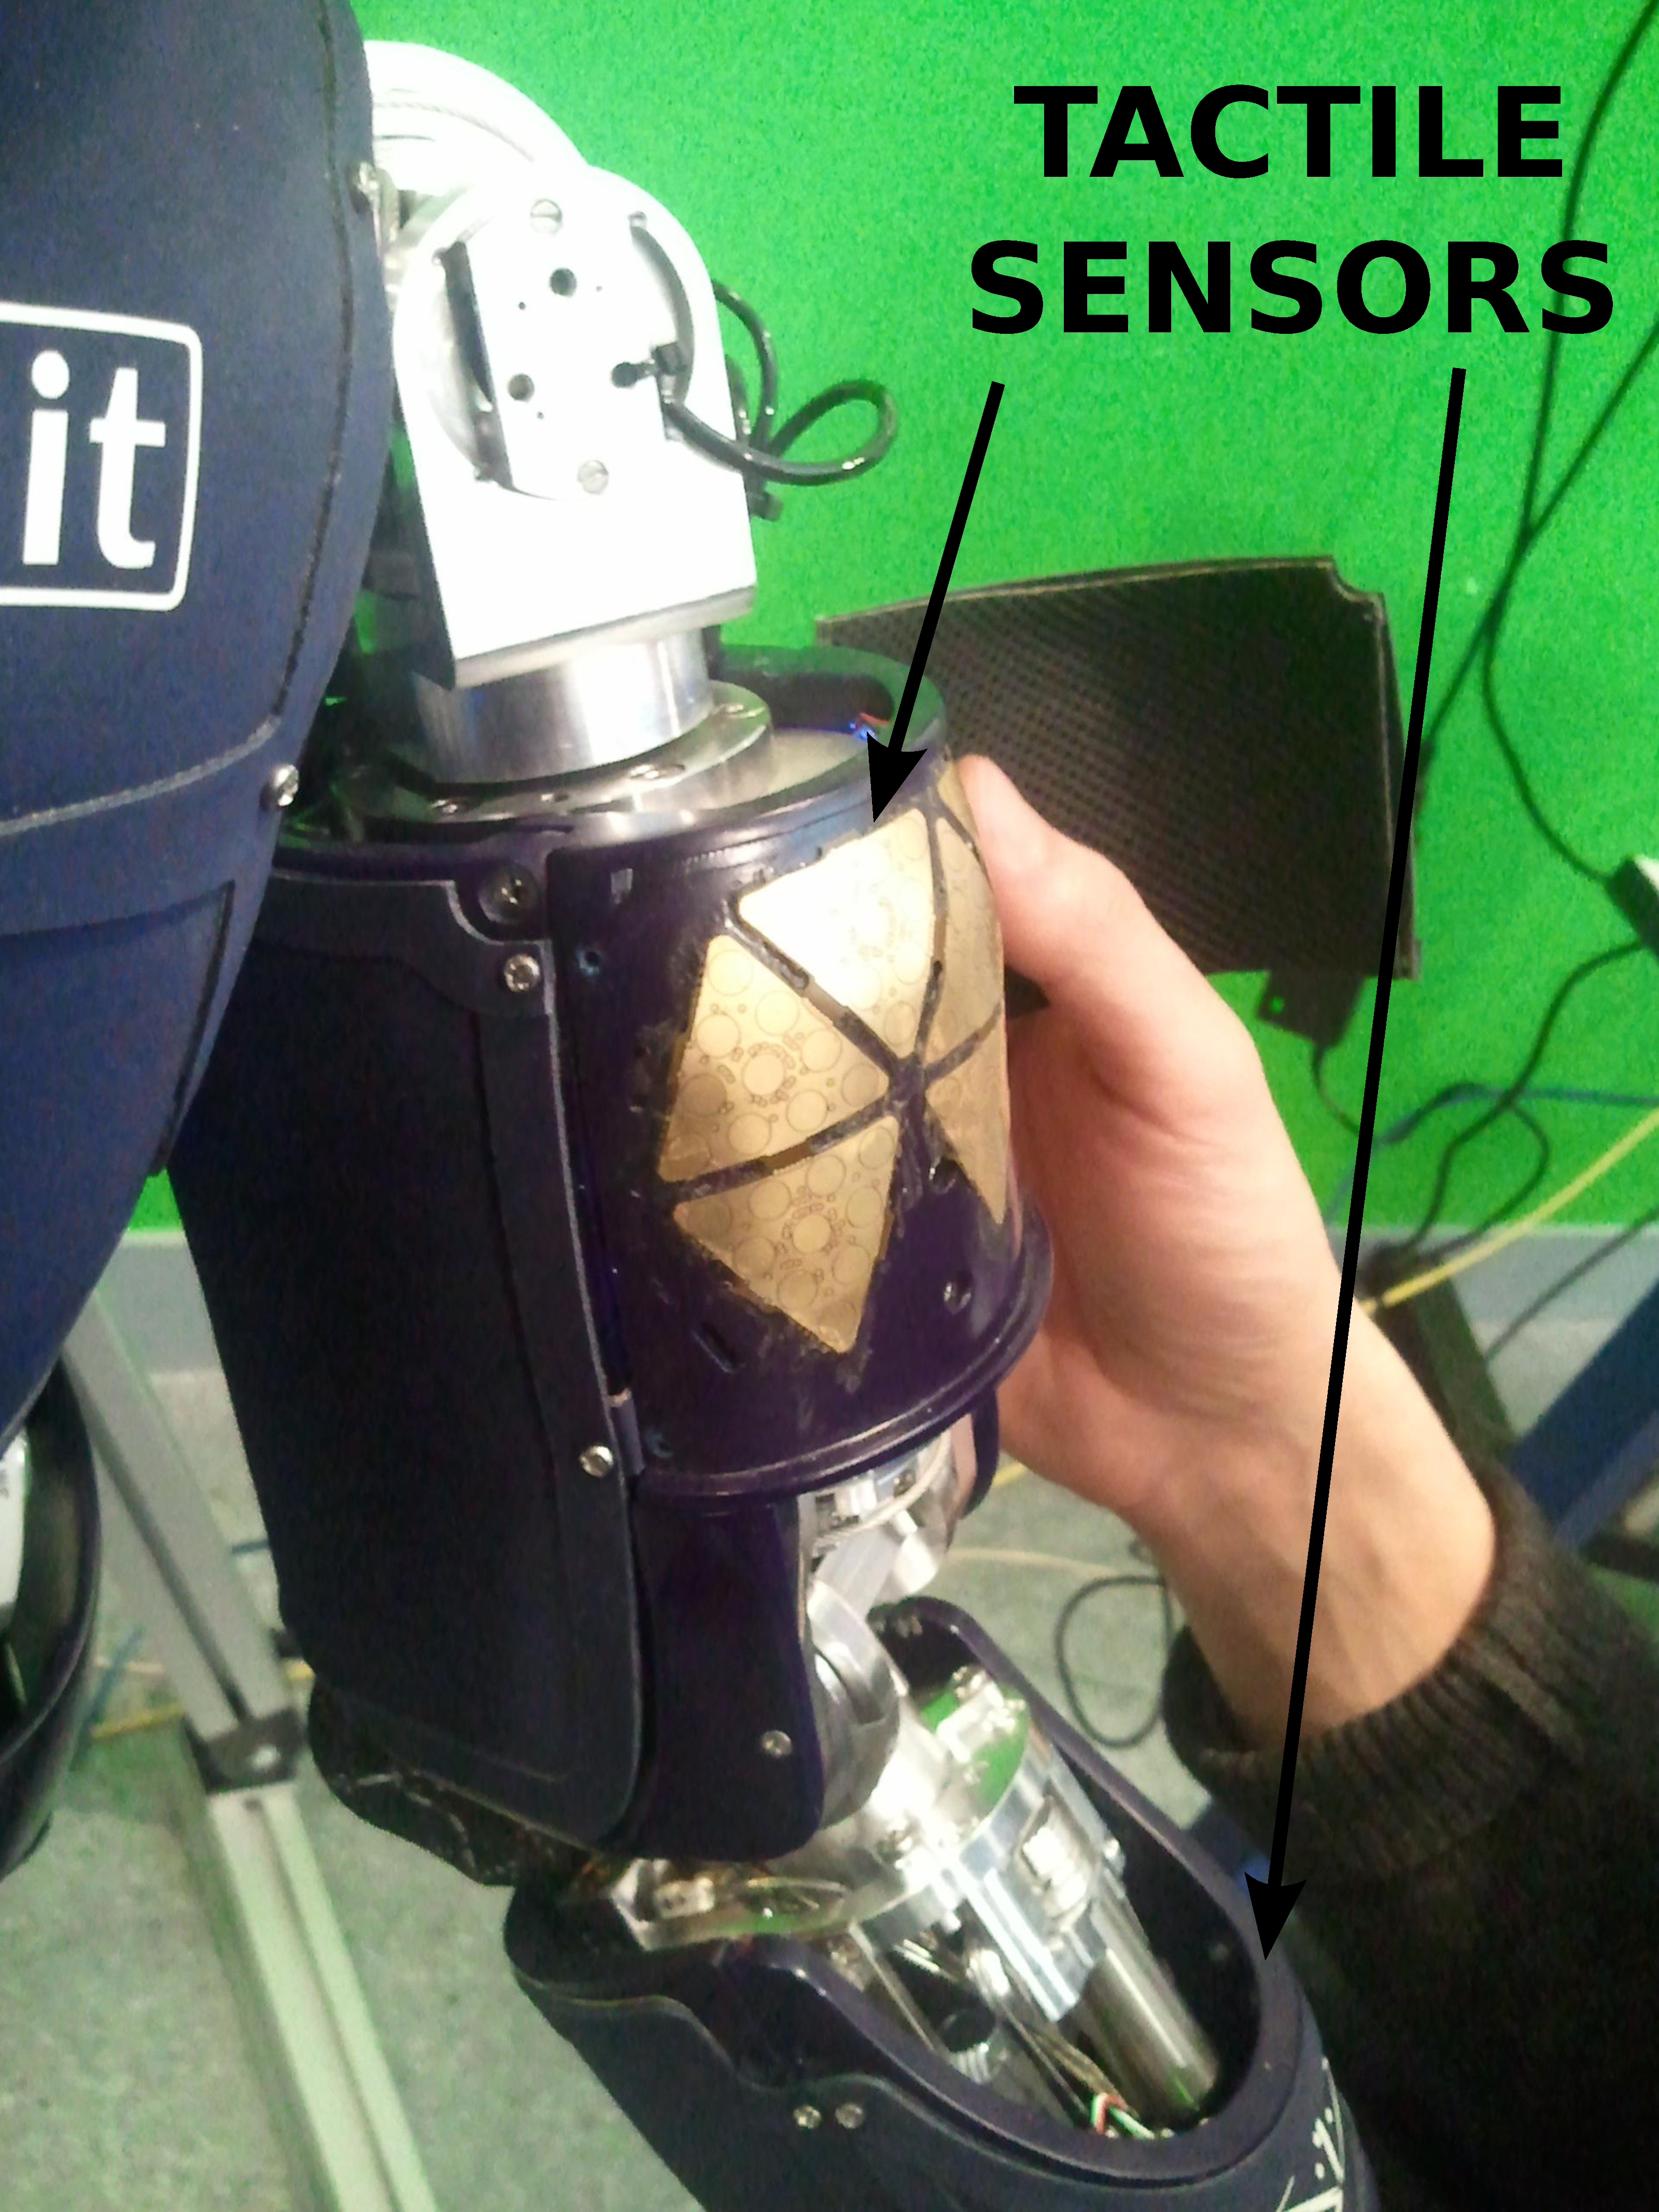
\includegraphics[height=4cm]{fig/icub_arm_skin_text}
% 	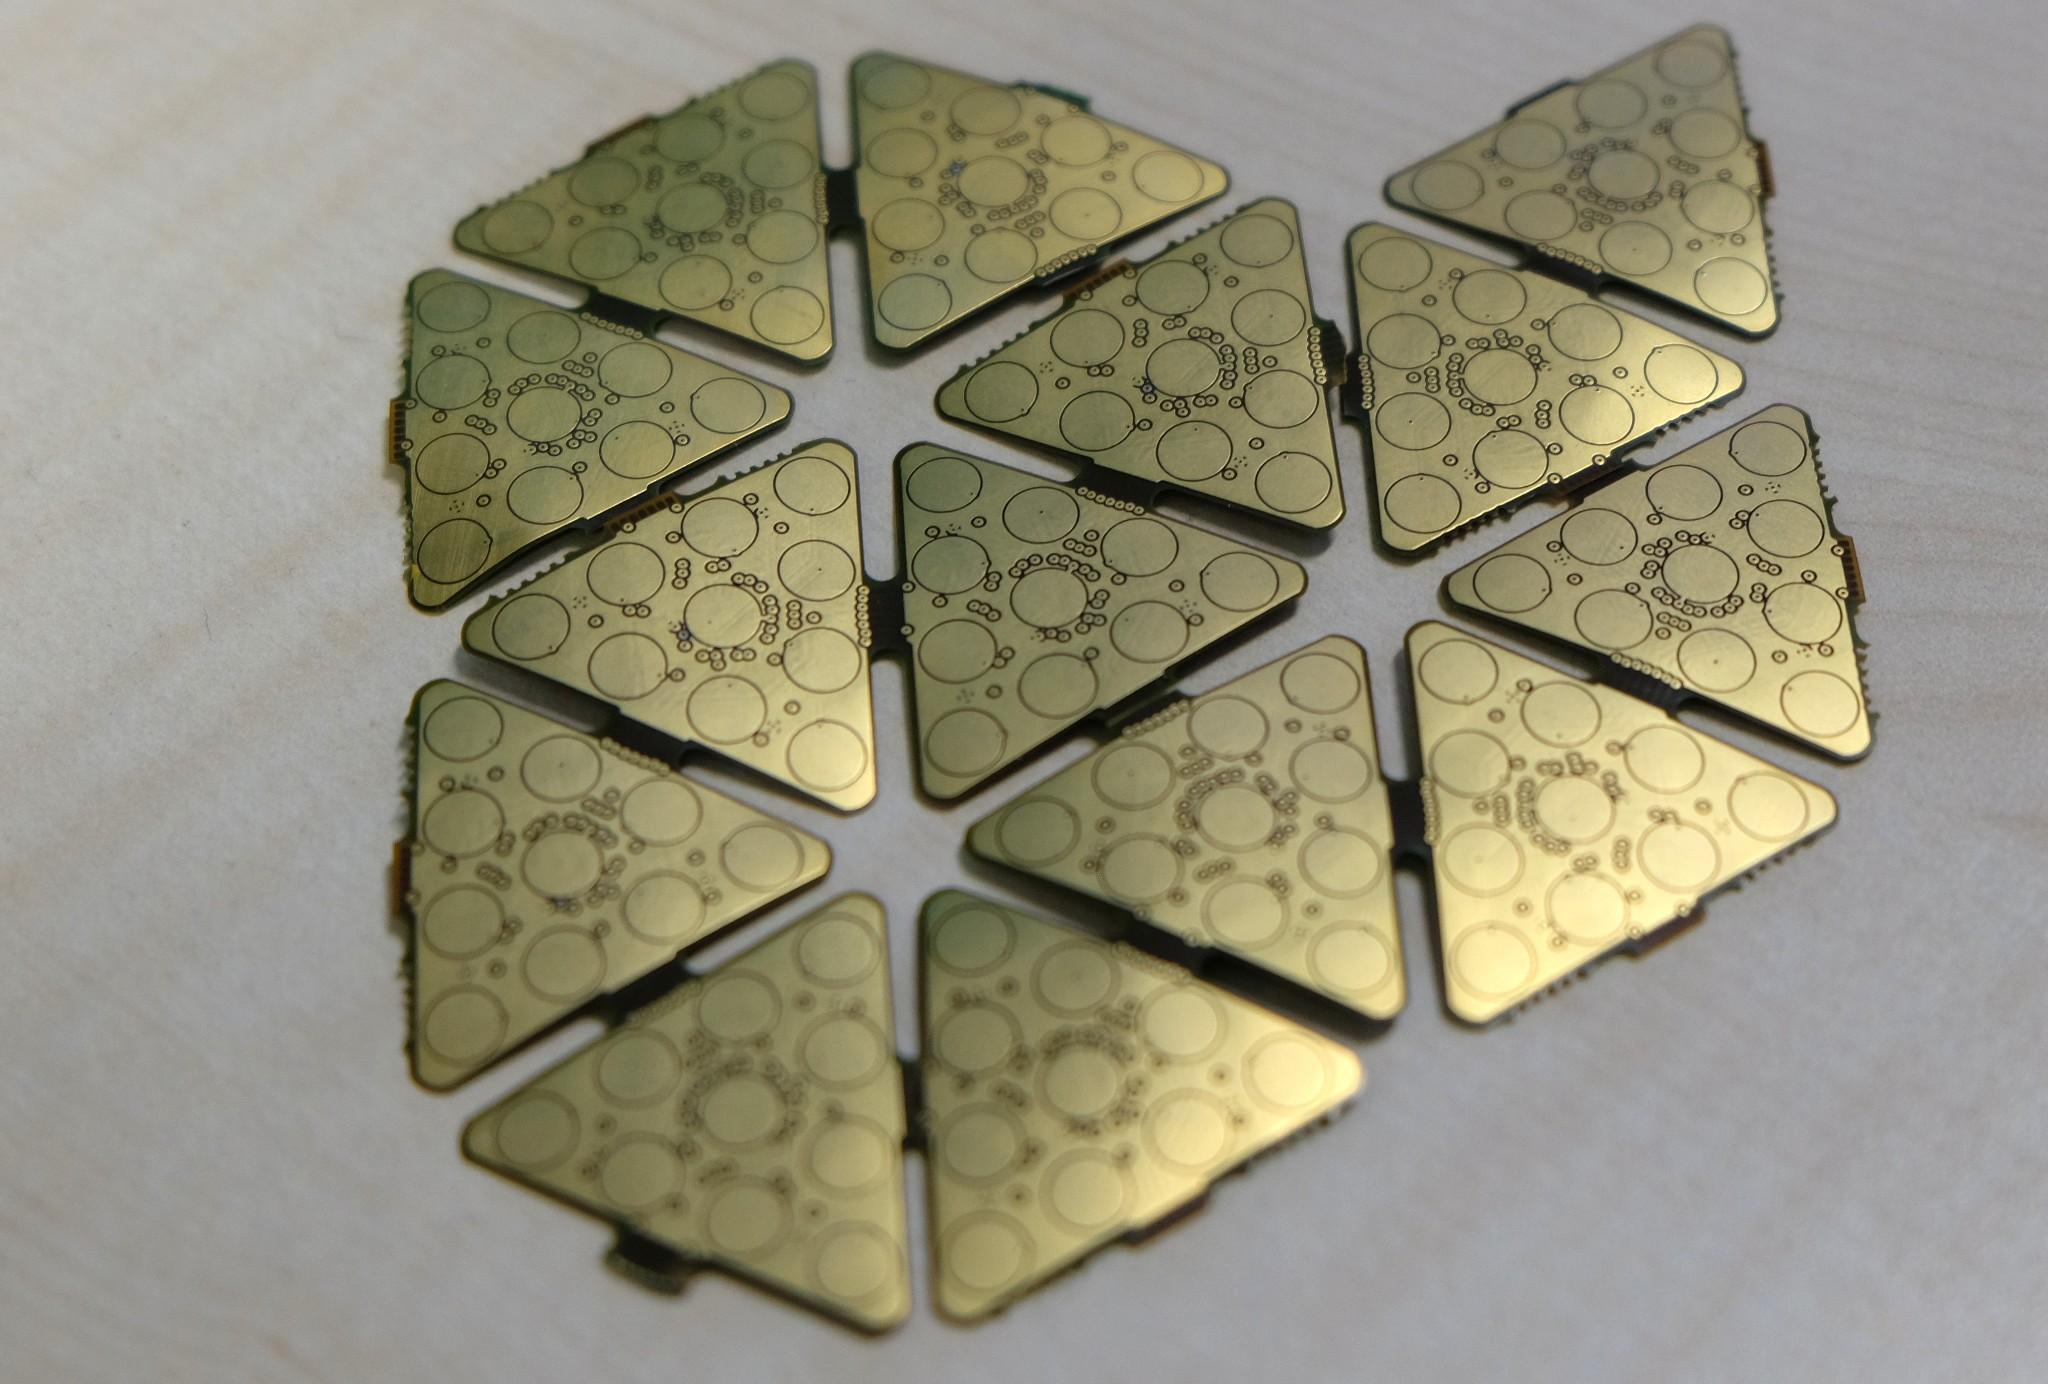
\includegraphics[height=4cm]{fig/Skin1b}
% 	\hfill
% 	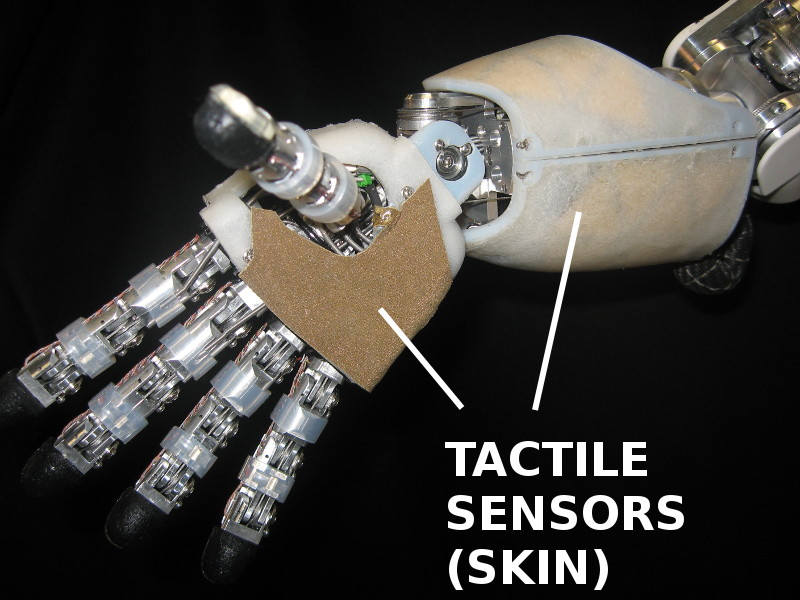
\includegraphics[height=4cm]{fig/icub_skin_arm_3}
% }
% 	\caption{The tactile elements (taxels) of the artificial skin covering the \robot{} arm. 
% 	Their measurements~$\skinInput$ are used to choose the appropriate expert.}
% 	\label{fig:icubskin}
% \end{figure}
%

%
	\begin{figure}[t]
		\centering
		\begin{subfigure}[t]{0.48\hsize}
			\centering
			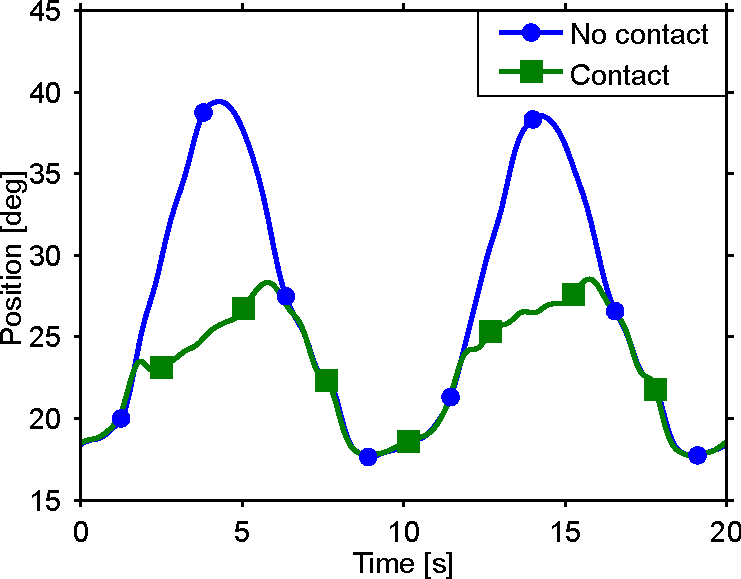
\includegraphics[height=3.2cm]{robertoICRA/fig/exp1_effectContactQ}%[width=.99\columnwidth]{fig/exp1_effectContactQ}
			\caption{Task space}
			\label{fig:exp1:effects_contact:a}
		\end{subfigure}
		\hfill
		\begin{subfigure}[t]{0.48\hsize}
			\centering
			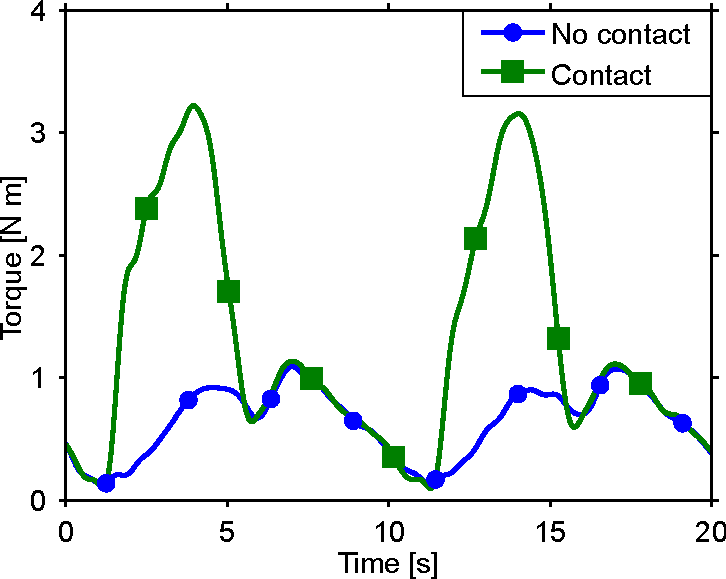
\includegraphics[height=3.2cm]{robertoICRA/fig/exp1_effectContactT}
			\caption{Torque}
			\label{fig:exp1:effects_contact:b}
		\end{subfigure}
		\caption{\textbf{\nameref{sec:results:exp1}:} Effects of a contact (green curve) compared to the free movement without obstacle (blue curve). 
		These effects are visible in the task space position~\subref{fig:exp1:effects_contact:a} and in the torque measured by the joint torque sensor~\subref{fig:exp1:effects_contact:b}.
		%\comment{Figures generated by \textit{Figures\_exp1}}
		}
		\label{fig:exp1:effects_contact}
        \figspace
	\end{figure}
	%


%% RESULTS
%we present the experimental results obtained.
 In this section, we describe the experimental setting and the humanoid robot~\robot{} used in the experiments.
% In the first experiment, we consider the case of learning a contact model for a fixed object. 
% In the second experiment, we demonstrate that a single contact model have generalization capabilities relatively to limited changes in the position of the contact.
% In the third experiment, we consider the case of multiple contacts. 
% We demonstrate that by combining models of single contacts it is possible to generalize to multiple contacts.
% In the fourth experiment, we consider a special case of multiple contacts: multiple simultaneous contacts.
% We show that our approach allows to sum the contributions from the single contacts to predict simultaneous multiple contacts.
% In the fifth experiment, we demonstrate that learning the gating network greatly reduce the design complexity, while achieve similar performances compared to a manual design.
%
We present four different experiments where we demonstrate that
1) Our approach can learn single contact models;
2) A single learned model (i.e., an expert) is robust to small changes in the position of the contact;
3) Our approach extends to multiple contacts by combining models of single contacts;
%4) our approach works even for multiple simultaneous contacts;\todo{check}
4) The gating network activating the experts can be learned to reduce the complexity of manually design it.

%===============================================================================


	

	

\subsection{Experimental set-up}

	%	
% 	\begin{wrapfigure}{r}{0.46\columnwidth}
% 	%\begin{figure}[t]
% 		\centering
%         \vspace{-10 pt}
% 		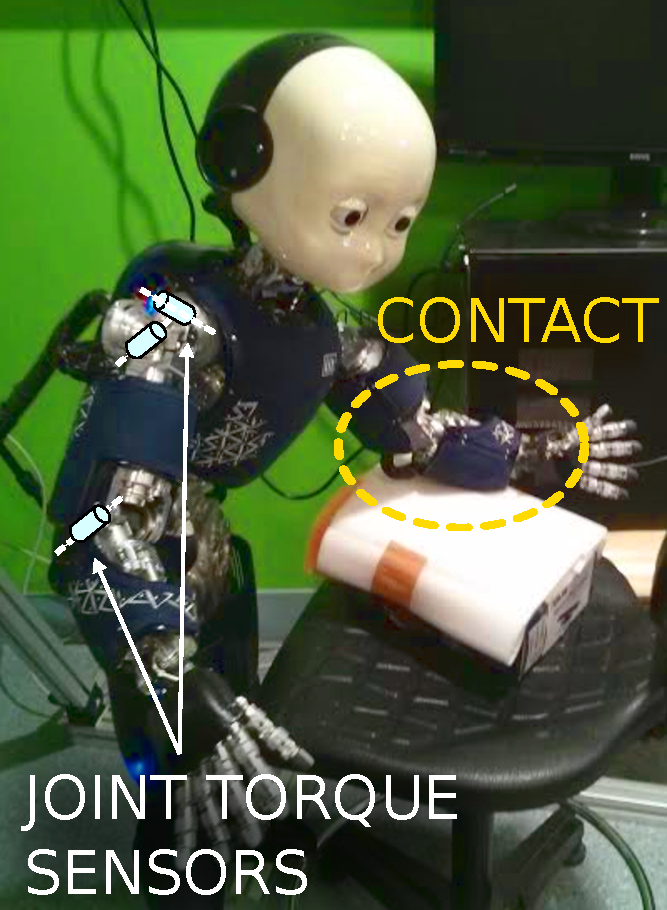
\includegraphics[width =\linewidth]{robertoICRA/fig/iCubParis02_contact_JTS}
% 		\caption{An experiment performed with iCub. The arm collides with the environment: the contact location is perceived by the skin in the forearm. On the left arm, the location of the three joint torque sensors is indicated.}
% 		\label{fig:icuparis_contact_jts}
% 	%\end{figure}
% 	\end{wrapfigure}
	%
	The experiments were conducted on the \robot{}~\cite{Natale2013}, a humanoid robot with 53 degrees of freedom, sized as a child (104 cm tall, 24 kg of weight).
	This robot is equipped with several sensors: an inertial sensor in the head, four 6-axis force/torque sensors placed proximally in the middle of legs and arms, and an artificial skin consisting of many distributed tactile elements (taxels) mounted on the robot covers~\cite{Cannata2008}. 
	The information from these three types of sensors is used to estimate the joint torques and the external contact forces by the \idyn{}  library~\cite{Ivaldi2011}. 
	In the following, $\torques_{\rm IDYN}$ denotes the joint torques estimated by the \idyn{} library, which we use as analytical model for comparison. 
	For more detail on its contact detection and taxels calibration we refer to~\cite{DelPrete2011,DelPrete2012}.
	%\comment{Still missing the explanation about why iDyn with multiple contacts is bad}

%	These sensors are used to detect the contacts, compute the external contact forces and estimate the joint torques~\cite{Fumagalli2012}. 
%	The tactile elements in the skin (see \fig\ref{fig:icubskin}) provide the information about the contact location; they also provide an indirect measure of the external force. 
%	The force/torque sensors, placed proximally in the middle of legs and arms, are used to estimate the robot dynamics (internal/external wrenches) and the joint torques.
%	This estimation is performed online by the library iDyn, which relies on the known dynamic model of the robot~\cite{Ivaldi2011}. 
%	\comment{Discuss the assumptions of the analytic model: ellipsoid thing}

 
	%Only one \robot{} was equipped with some joint torque sensors: precisely, iCubParis02 has three, placed in the first, second and fourth joint of the arm. 
	The \robot{} used in the experiments is equipped with three additional Joint Torque Sensors (JTSs), two in the shoulder and one in the elbow.
	The JTSs are calibrated by computing the offset and gain trough least-square regression with respect to the output of~\idyn{}.
	We consider these calibrated JTSs as ground truth measurements of the joint torques~$\jtsForces$.
	%\fixme{To calibrate the JTS, we compute the offset as the difference in absence of movement and the gain using Least-Square regression on the data.}
	%%The \robot ~\cite{Metta2008} is a humanoid robot with \fixme{N} degrees of freedom.
	%These skin sensors measure values correlated with the pressure applied to the skin itself.
	%
    	In our experiments, we used the \robot{} torso and arms (3 and 7 degrees of freedom, respectively) and the skin input~$\skinInput$ from the forearm, which consists of 270 sensor measurements.


%===============================================================================

%
	\begin{figure}[t]
		\centering
		\begin{subfigure}[t]{0.48\hsize}
			\centering
			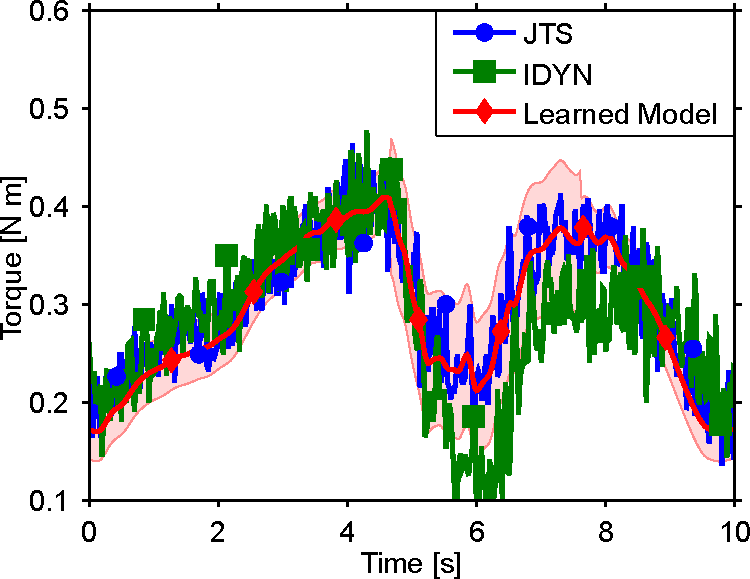
\includegraphics[width=.69\columnwidth]{robertoICRA/fig/exp1_model_notfilt}
			\caption{Real data.}
			\label{fig:exp1:model_contact:a}
		\end{subfigure}
		\hfill
		\begin{subfigure}[t]{0.48\hsize}
			\centering
			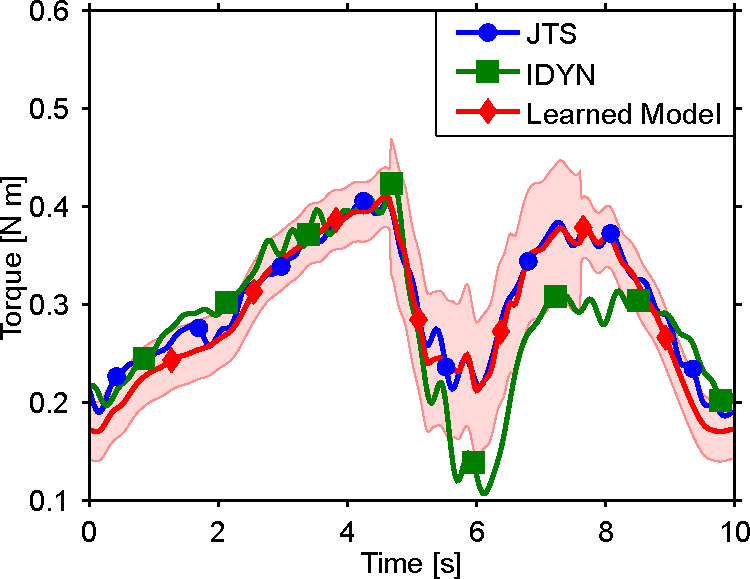
\includegraphics[width=.69\columnwidth]{robertoICRA/fig/exp1_model_filt}
			\caption{Filtered visualization.}
			\label{fig:exp1:model_contact:b}
		\end{subfigure}
		\caption{\textbf{\nameref{sec:results:exp1}}: Comparison of the torque measured at the elbow (with contact) by the JTS,  estimated by \idyn{} and our learned model (shown as $\text{mean}\pm 2\,\text{std}$). 
		Our learned model better predict the torque measured by JTS~\subref{fig:exp1:model_contact:a}.
		Additionally, due to the identification of the noise in the model, its prediction is smoother compared to both the noisy JTS measurements and the prediction from \idyn{}.
		For visualization purposes we also show the predictions when filtering JTS and \idyn{}~\subref{fig:exp1:model_contact:b}.
		%\comment{Figure generated by \textit{SomeFigures}}
		}
		\label{fig:exp1:model_contact}
        \figspace
	\end{figure}
	%
    	% 
	\begin{table}[t]
		\resizebox{\hsize}{!}{
		\centering
		\begin{tabular}{|l|l|c|c|c|}
			\hline 
			& Method	& Shoulder 1 [Nm] & Shoulder 2 [Nm] & Elbow [Nm] \\
% 			\cline{2-7}
			\hline 	
			\multirow{2}{*}{Full trajectory}  & \idyn{} & $0.09 \pm 1.1 \times 10^{-3}$ & $0.16 \pm 1.8 \times 10^{-3}$ & $0.05 \pm 7.4\times 10^{-4}$ \\ 
			& Our model 		& $\mathbf{0.04  \pm 5.6 \times 10^{-4}}$ & $\mathbf{0.07  \pm 9.8\times 10^{-4}}$ & $\mathbf{0.02  \pm 3.1\times 10^{-4}}$ \\
			\hline
			\multirow{2}{*}{Contact only}  & \idyn{} 	& $0.07 \pm 3.1 \times 10^{-3}$ & $0.13 \pm 5.7 \times 10^{-3}$ & $0.08 \pm 3.0 \times 10^{-3}$\\ 
			& Our model 		& $\mathbf{0.03  \pm 1.5 \times 10^{-3}}$ & $0.12  \pm 5.9 \times 10^{-3}$ & $\mathbf{0.03  \pm 1.3 \times 10^{-3}}$ \\
			%\cline{2-7}
			\hline
		\end{tabular}
		}
		\caption{\textbf{\nameref{sec:results:exp1}:} Mean and standard deviation of the mean for the RMSE of the test set for ground truth, predictions with the \idyn{} and our learned model. 
		The learned model predicts the torque more accurately than~\idyn{} for both the full trajectory and  during the only contact phase.
		}
		\label{tab:exp1}
        \figspace
	\end{table}
	%

\subsection{Learning a single contact}
\label{sec:results:exp1}


	In this experiment, we consider the \robot{} making contact with a single obstacle.
	%
	%% objectives of the experiment
	The evaluation is performed on a simple tracking task with the \robot{}'s end-effector moving along a circular trajectory.
	We repeat the task twice: first without any contact and then with a contact at a fixed position.
\fig\ref{fig:exp1:effects_contact} shows the effects of the contact in terms of position and torque during the tracking task. When the contact occurs the position error increases considerably. As a result, the torque is increased to compensate for the obstacle. 
	We collected 10 repetitions of the trajectory with the contact and used 8 of them to train the model.
    %We down-sampled the data to 40 Hz for a total of 939 data points, in order to reduce the computational time.
	The remaining trajectories are used as test set to evaluate the predictive performances of our learned model.
    For this experiment we consider a single expert (the gating network still decides whether to activate the expert).
    
    
    %We assess the quality of a learned contact model compared to the classical inverse dynamics model $\torques(\q,\dq,\ddq)$.
	We compare the baseline joint torque (measured by the JTS) to the joint torque estimated by the analytic model \idyn{} and  the joint torque $\torques_\text{IDM}$ predicted by our learned model.
	In \tab\ref{tab:exp1}, we report the root mean square error (RMSE) and the standard deviation of the mean of \idyn{} and our learned model for all the three joints.
	Additionally, we report both the error of the learned models (learned RBD plus learned contact model) during the full trajectory and exclusively \textit{during} the contact. 
	In five out of six cases, the learned model performs better than the analytic model. 
    In the sixth case (contact only, shoulder 2), the performance of the learned model is similar to the analytic model.
    However, increasing the amount of data used for training may further increase the performance of the learned model. 
    %\todo[inline]{Sounds funny: it's only similar because of small training data set size. Otherwise it should be worse? BTW: what is the training set size?}
	%We hypothesize that the performance of the learned model is due to the limited amount of data used for training.
	%In the following experiments, where more data was collected, the prediction accuracy for shoulder 2 improves in line with shoulder 1 and the elbow.
	%Failing to do so, would further decrease the performances of \idyn{}, due to the previously mentioned prediction error in the RBD.
	A visual representation of the predictions of the test set for the elbow joints is shown in~\fig\ref{fig:exp1:model_contact}.
	
    This experiment provides evidence that the classical rigid-body dynamics model $\torques_\text{RBD}(\q,\dq,\ddq)$ and the \idyn{} estimation (that also exploits proximal force/torque sensing) fail to accurately estimate the joint torques when the robot is in contact with the environment. 
	%Therefore, we need to include the contact information in such a model, i.e., $\torques_\text{IDM}(\q,\dq,\ddq,\skinInput,\ftsForces)$.
	Moreover, we show that the learned contact model, when combined with the RBD model, provides a better approximation of the joint torque.
	

% 	%
% 	\begin{figure}[t]
% 		\centering
% 		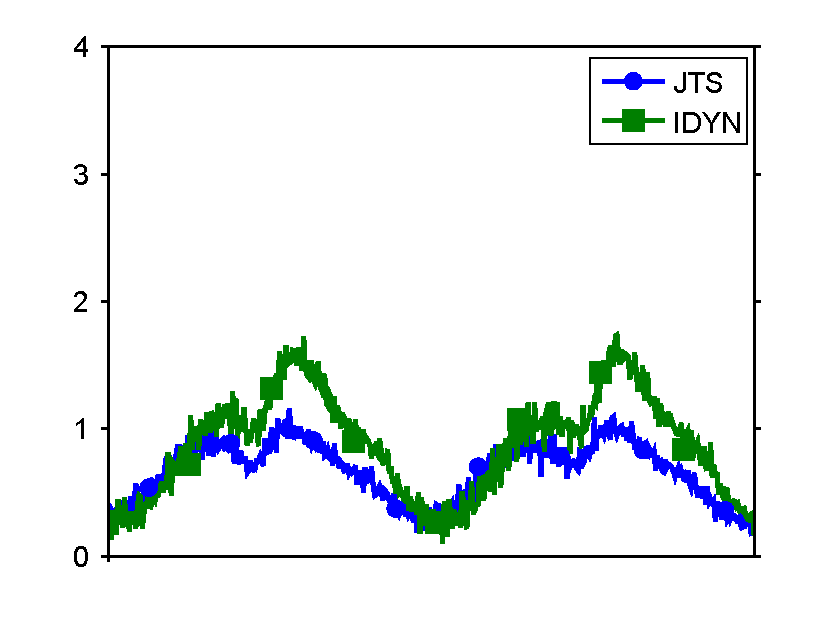
\includegraphics[width=.99\columnwidth]{robertoICRA/fig/exp1_contact}
% 		\caption{\textbf{\nameref{sec:results:exp1}}: the comparison, in absence of contact, of the torque measured by the JTS, the one estimated by iDyn using the FTS and the one generated by combining the RBD model with the learned model. \comment{Figure generated by \textit{SomeFigures}}}
% 		\label{fig:exp1:model_nocontact}
% 	\end{figure}
% 	%



%===============================================================================


\subsection{Robustness of the single contact model}
\label{sec:results:exp2}

% %
% 	%\begin{figure}[t]
% 		\begin{figure}[t]
% 		\begin{minipage}{.46\linewidth}
% 		\centering
% 		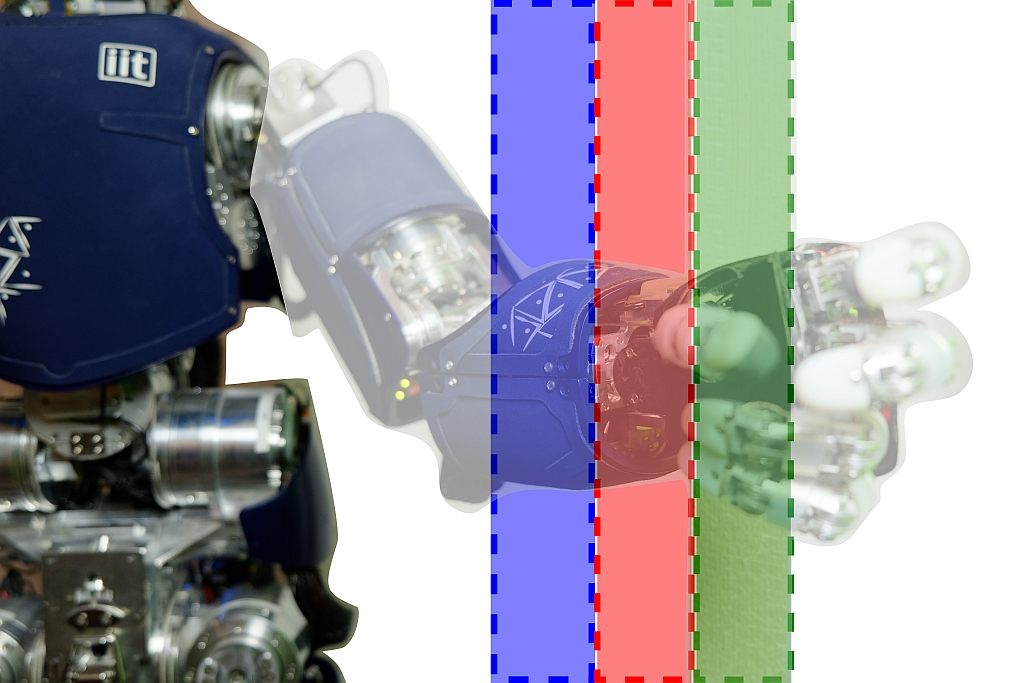
\includegraphics[width=.99\hsize]{robertoICRA/fig/Generalized_01}
% 		\caption{\textbf{\nameref{sec:results:exp2}}: The robot performs a movement with the left arm. The forearm collides with one of the three different obstacle: \textcolor{blue}{contact 1 (far)}, \textcolor{red}{contact 2 (medium)} or \textcolor{darkgreen}{contact 3 (close)}}
% 		\label{fig:exp2:robot}
% 	%\end{wrapfigure}
% 	%\end{figure}
% 	%
% 	\end{minipage}
% 	\hfill
% 	\begin{minipage}{.50\linewidth}
% 	 	%
%  	%\begin{figure}[t]
% 		\centering
% 		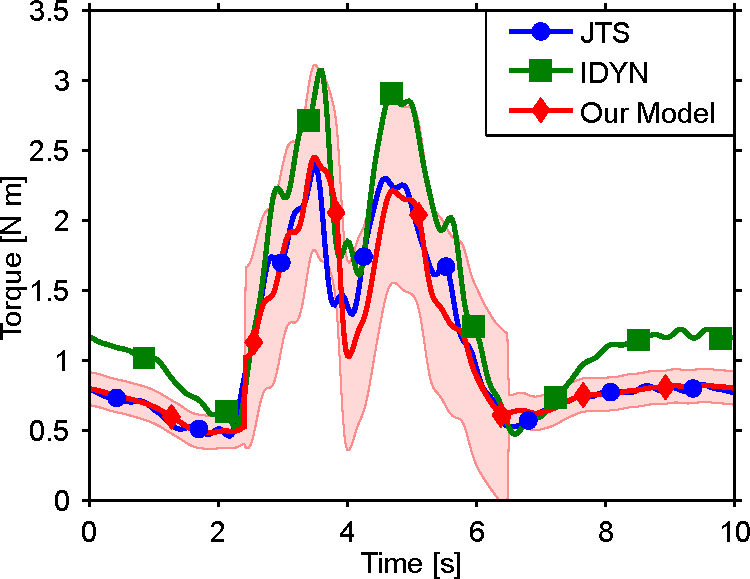
\includegraphics[width=.99\hsize]{robertoICRA/fig/exp2_model}
% 		\caption{\textbf{\nameref{sec:results:exp2}}: Prediction for the \textcolor{red}{medium contact} on the joint \textit{shoulder 2} (for visualization purposes JTS and \idyn{} are filtered).
% 		Even if a contact in this position was not observed during learning, the single contact model was robust to small variations in the position of the obstacle.}
% 		\label{fig:exp2:model_contact}
% 		\end{minipage}
% 	\end{figure}
% 	%
	
	%
	\begin{figure}[t]
		\resizebox{\hsize}{!}{
		\centering
		\begin{subfigure}[t]{0.48\hsize}
			\centering
			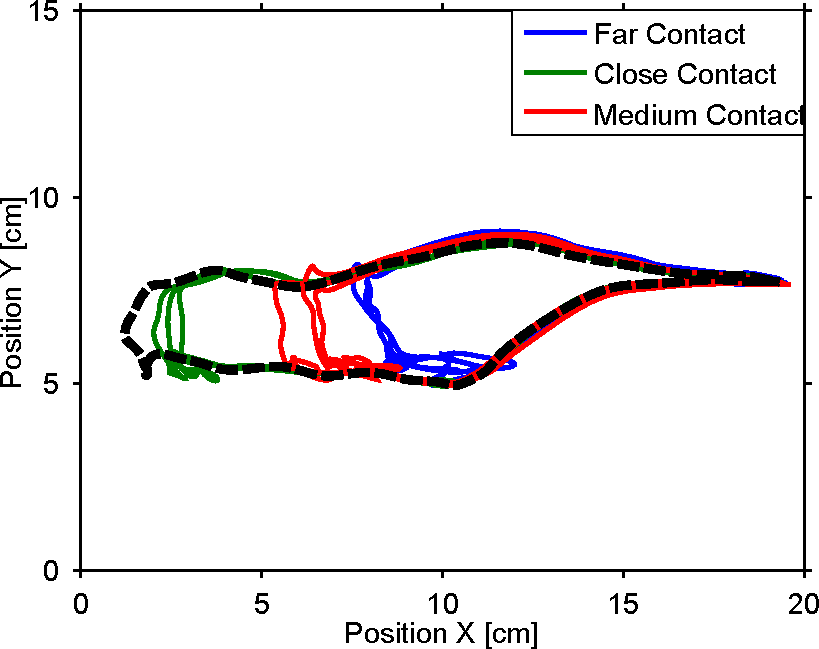
\includegraphics[height=4.2cm]{robertoICRA/fig/generalized_contact_a.pdf} %[width=.99\columnwidth]
			\caption{Task space}
			\label{fig:effects_contact:a}
		\end{subfigure}
		\hfill
		\begin{subfigure}[t]{0.48\hsize}
			\centering
			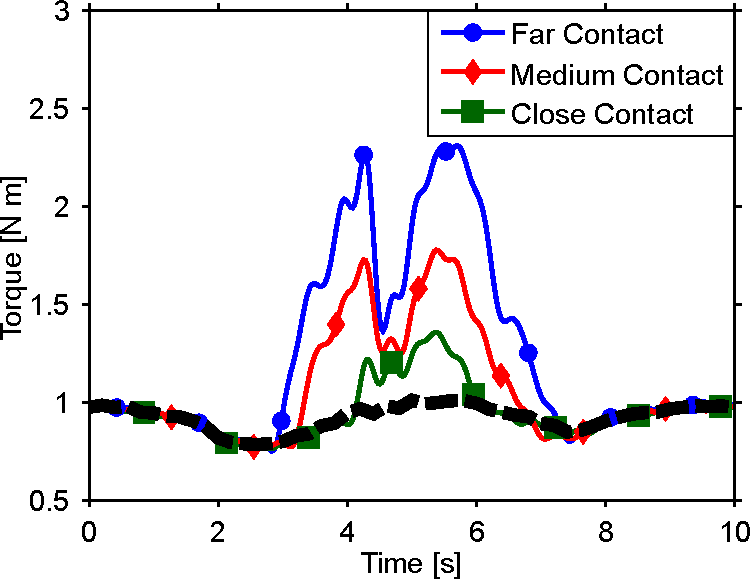
\includegraphics[height=4.2cm]{robertoICRA/fig/generalized_contact_b.pdf} % [width=.99\columnwidth]
			\caption{Torque}
			\label{fig:effects_contact:b}
		\end{subfigure}
		}
		\caption{\textbf{\nameref{sec:results:exp2}:} Effects of the contact on the task space and the torque for the three different contact types: contact 1 (far), contact 2 (medium) and contact 3 (close). 
		The task in absence of contact is displayed as reference (\textbf{black dashed curve}). 
		%\comment{Figures generated by \textit{Figures\_exp2}}
		}
		\label{fig:exp2:effects_contact}
        \figspace
	\end{figure}
	%
	
	
%\todo{say about no gating network}
	%We now extend the single contact experiment to cover generalized single contacts.\todo{what is a generalized contact?}
	In the following, we show that the prediction performance of each GP expert is robust to small variations in the position of the contact.
	This is important since the exact position of the obstacle does not need to be known in advance (within a single expert $f_j$).
	As in the previous experiment we consider a tracking task along a circular trajectory.
	However, this time the obstacle is placed at one of three different positions along the trajectory: close, medium and far.
    Each of these obstacles is shifted 2\,cm along the horizontal axis.
	Obstacles at different positions along the trajectory lead to different effects in terms of both joint position and torque signal, as clearly visible in~\fig\ref{fig:exp2:effects_contact}.
	Note that the skin input~$\skinInput$ will also be affected, as shown in~\fig\ref{fig:exp2:skin}. 
    Hence, we could potentially learn a separate expert for each contact. 
    However, we only consider a single expert as we want to demonstrate the robustness of a single expert, not of the gating network.
	%Therefore, we assume that the gating network has been appropriately devised to consider the three different contacts as belonging to the same family of contacts, rather than three different contacts.
    
    %
	\begin{figure}[t]
		\centering
		\begin{subfigure}[t]{0.30\hsize}
        \centering
			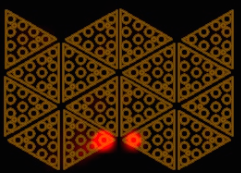
\includegraphics[height=1.8cm]{robertoICRA/fig/paris2_new} 
			\caption{Contact 1}
		\end{subfigure}
		\hspace{0.1cm}
		\begin{subfigure}[t]{0.30\hsize}
        \centering
			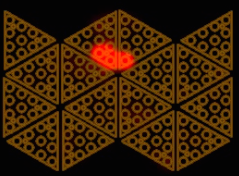
\includegraphics[height=1.8cm]{robertoICRA/fig/paris3_new} 
			\caption{Contact 2}
		\end{subfigure}
		\hspace{0.1cm}
		\begin{subfigure}[t]{0.30\hsize}
        \centering
			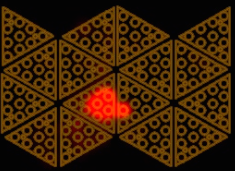
\includegraphics[height=1.8cm]{robertoICRA/fig/paris7_new}
			\caption{Contact 3}
		\end{subfigure}
		\caption{\textbf{\nameref{sec:results:exp2}}. The different contact locations detected by the forearm skin respectively for the three contacts: contact~1 (far), contact~2 (medium) and contact~3 (close).}
		\label{fig:exp2:skin}
        \figspace
	\end{figure}
	%

	% 
	\begin{table}[t]
		\resizebox{\hsize}{!}{
		\centering
		\begin{tabular}{|l|l|c|c|c|}
			\hline 
			& Method	& Shoulder 1 [Nm] & Shoulder 2 [Nm] & Elbow [Nm] \\
			\hline 	
			\multirow{2}{*}{Far contact}  & \idyn 	& $0.13 \pm 3.9 \times 10^{-3}$  &  $0.40 \pm 9.7\times 10^{-3}$ & $0.06 \pm 1.9\times 10^{-3}$ \\ 
			&Our model 		& $\mathbf{0.06  \pm 1.9\times 10^{-3}}$ & $\mathbf{0.08  \pm 2.9\times 10^{-3}}$ & $\mathbf{0.03  \pm 8.0 \times 10^{-4}}$\\
			\hline 	
			\multirow{2}{*}{Close contact}  & \idyn 	& $0.09 \pm 2.2\times 10^{-3}$ & $0.22 \pm 4.5\times 10^{-3}$ & $0.04 \pm  0.9\times 10^{-3}$\\ 
			&Our model 		& $\mathbf{0.06  \pm 1.4\times 10^{-3}}$ & $\mathbf{0.06 \pm 1.4\times 10^{-3}}$ & $\mathbf{0.02  \pm 6.3\times 10^{-4}}$ \\ % 0.58 0.58 is correct!
			\hline 	
			\multirow{2}{*}{Medium contact}  & \idyn 	& $0.10 \pm 2.8\times 10^{-3}$ & $0.32 \pm 6.7\times 10^{-3}$ & $0.05 \pm 1.3\times 10^{-3}$ \\ 
			&Our model 		& $\mathbf{0.06 \pm 1.7\times 10^{-3}}$ & $\mathbf{0.12 \pm 4.7\times 10^{-3}}$ & $0.05 \pm 1.7\times 10^{-3}$ \\
			\hline
		\end{tabular}
		}
		\caption{\textbf{\nameref{sec:results:exp2}:} Errors between the ground truth~(JTS) and the predictions with either the \idyn{} and our learned model on the test set. 
		A single expert is robust to small variations of the contact.
		}
		\label{tab:exp2}
        \figspace
	\end{table}
	%
    
    %\todo[inline]{Not sure what the experiment was doing that you described above. The notion of the gating network just appeared at the end.}
	%The contact model is learned using the data collected at 40 Hz from contact 1 and contact 3 (far and close contacts), summing up to a total of 978 data points.
    The contact model is learned using the data collected from contact 1 and contact 3 (far and close contacts) and as validation the data set generated from the \textit{unseen} contact 2 (medium) is used.
	%\comment{Describe dataset: 978 datapoints, 40 Hz}
	%We learn a model using the collected data from two of the obstacles (close and far), and test the resulting model on the third (medium) \textit{unseen} obstacle.
	In \tab\ref{tab:exp2}, the RMSE for all three contacts are reported for \idyn{} and our learned model, respectively.
	The results show that the learned model is robust to unseen contacts and performs  equally well or better than the analytic model \idyn{}. 
	%\fig\ref{fig:exp2:model_contact} shows an example of the prediction for the unseen contact.



%===============================================================================


\subsection{Learning multiple contacts}
\label{sec:results:exp3}


   
% 	%
% 	\begin{figure}[t]
% 		\centering
% 		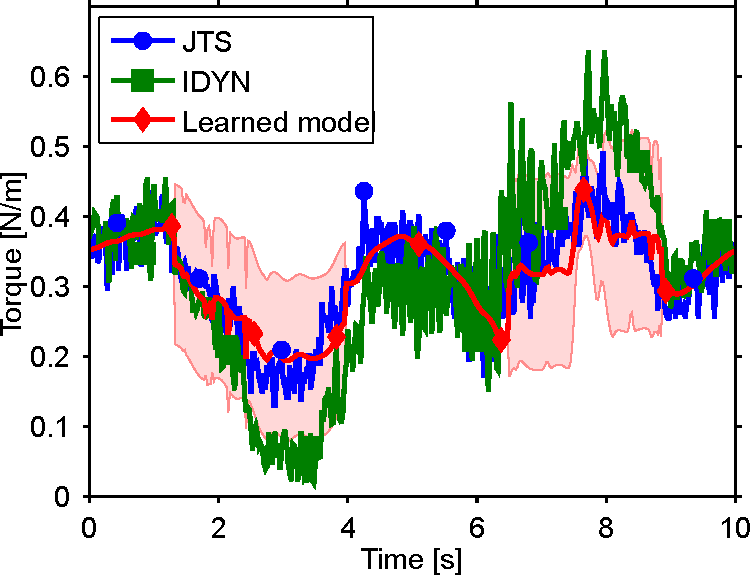
\includegraphics[width=.60\linewidth]{robertoICRA/fig/exp3_1}\\
% 		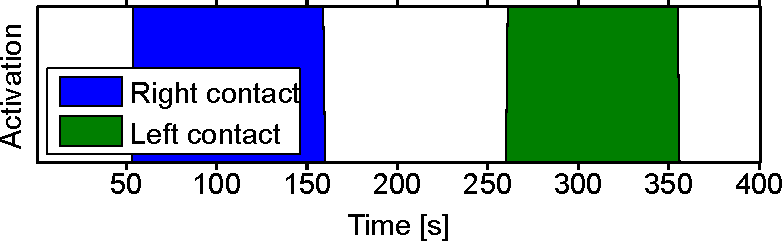
\includegraphics[width=.60\linewidth]{robertoICRA/fig/exp3_2}
% 		\caption{\textbf{\nameref{sec:results:exp3}:} Prediction of torques in presence of multiple contacts. 
% 		Various models are shown, but individually, none of them correctly capture the dynamics of the system. 
% 		Our approach combine them to successfully generalize to unseen configurations.
% 		}
% 		\label{fig:exp3:gating}
% 	\end{figure}
% 	%
		% 
	\begin{table}[t]
		\resizebox{\hsize}{!}{
		\centering
		\begin{tabular}{|l|l|c|c|c|}
			\hline 
			& Method	& Shoulder 1 [Nm] & Shoulder 2 [Nm] & Elbow [Nm] \\
			\hline 	
			\multirow{2}{*}{Right contact} & \idyn{} & $0.10\pm 1.3 \times 10^{-3}$ & $0.13\pm 1.6 \times 10^{-3}$ & $0.06\pm 8.1 \times 10^{-4}$ \\ 
			& Our model 		& $\mathbf{0.04\pm 6.3 \times 10^{-4}}$ & $\mathbf{0.07\pm 1.2 \times 10^{-3}}$ & $\mathbf{0.02\pm 2.7 \times 10^{-4}}$ \\
			\hline
			\multirow{2}{*}{Left contact}  & \idyn{} & $0.08 \pm 1.2 \times 10^{-3}$ & $0.16 \pm 2.0 \times 10^{-3}$ & $0.05 \pm 8.2 \times 10^{-4}$ \\ 
			& Our model 		& $\mathbf{0.03 \pm 5.7 \times 10^{-4}}$ & $\mathbf{0.07 \pm 9.6 \times 10^{-4}}$ & $\mathbf{0.02 \pm 2.8 \times 10^{-4}}$ \\
			\hline
			\multirow{2}{*}{Both contacts}  & \idyn{} & $0.10 \pm 1.3 \times 10^{-3}$ & $0.11 \pm 1.4 \times 10^{-3}$ & $0.07 \pm 8.4 \times 10^{-4}$ \\ 
			& Our model 		& $\mathbf{0.05\pm 8.3 \times 10^{-4}}$ & $\mathbf{0.10\pm 1.6 \times 10^{-3}}$ & $\mathbf{0.03 \pm 4.0 \times 10^{-4}}$ \\
			\hline
		\end{tabular}
		}
		\caption{\textbf{\nameref{sec:results:exp3}:} Root mean square error between the ground truth~(JTS) and the predictions with the \idyn{} and our learned model on the test set. 
		Our learned model predicts the torque more accurately than \idyn{}.
		}
		\label{tab:exp3}
        \figspace
	\end{table}
	%
	%
    After learning single contacts, we now show how to combine the learned models to adapt to unseen and more complex environments with multiple contacts.
	We consider a scenario having the \robot{} performing a circular motion with its left arm.
	%We initially generate a reference trajectory without any obstacle.
	We initially performed two experiments with an obstacle either on the left and on the right of the reference trajectory (see \fig\ref{fig:exp3:icuparis_experiment_bars}).
	%These obstacles clearly limit the motion of the end effector as shown in \fig\ref{fig:exp3:effects_contacts_pos:a} and \fig\ref{fig:exp3:effects_contacts_pos:b}.
	With the data collected in these two contact cases, we trained two independent expert models $f_1$, $f_2$, one for each contact.
	We repeated the experiment, but this time with both left and right contacts 
    %(see \fig\ref{fig:exp3:effects_contacts_pos:a}) 
    and used this last unseen case to validate our models. 
\fig\ref{fig:exp3:gating} shows an example of the prediction and the corresponding activation of the two contact models. 
	During both the right and the left contact, the corresponding experts are activated by the gating network.
	Therefore, we can successfully combine the contributions of the single contact models learned to generalize to unseen cases with multiple contacts.
	 \tab\ref{tab:exp3} reports the RMSE for the predictions.
     We notice that even in this experiment the experts accurately learn the effects of single contacts.
     Moreover, the gating network allows us to combine the experts to generalize to unseen environments, such as in the case of both contacts. 
     

%  	%
% 	\begin{figure}[t]
% 		\centering
% 		\begin{subfigure}[t]{0.32\hsize}
% 			\centering
% 			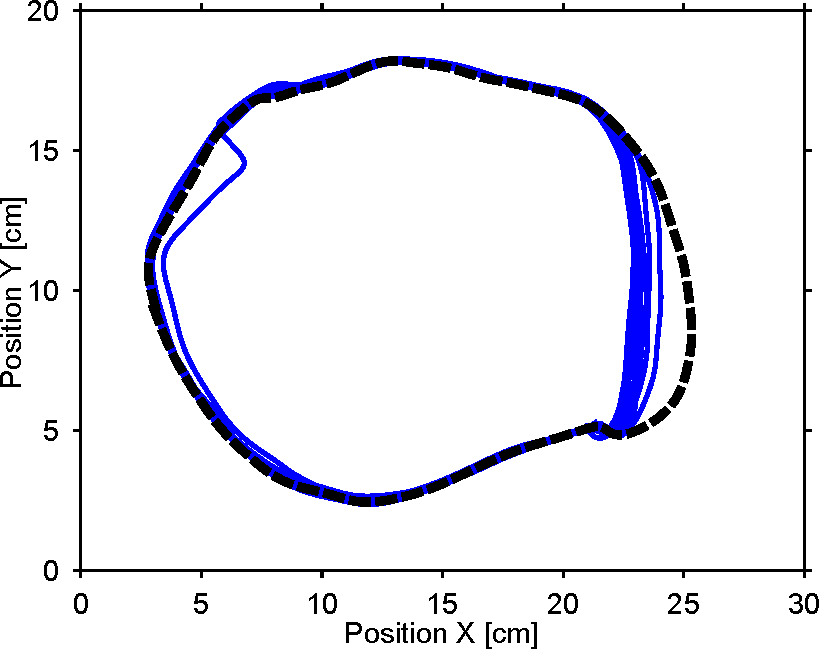
\includegraphics[width=.99\columnwidth]{robertoICRA/fig/Double_contact_a}
% 			\caption{Right contact}
% 			\label{fig:exp3:effects_contacts_pos:a}
% 		\end{subfigure}
% 		\hfill
% 		\begin{subfigure}[t]{0.32\hsize}
% 			\centering
% 			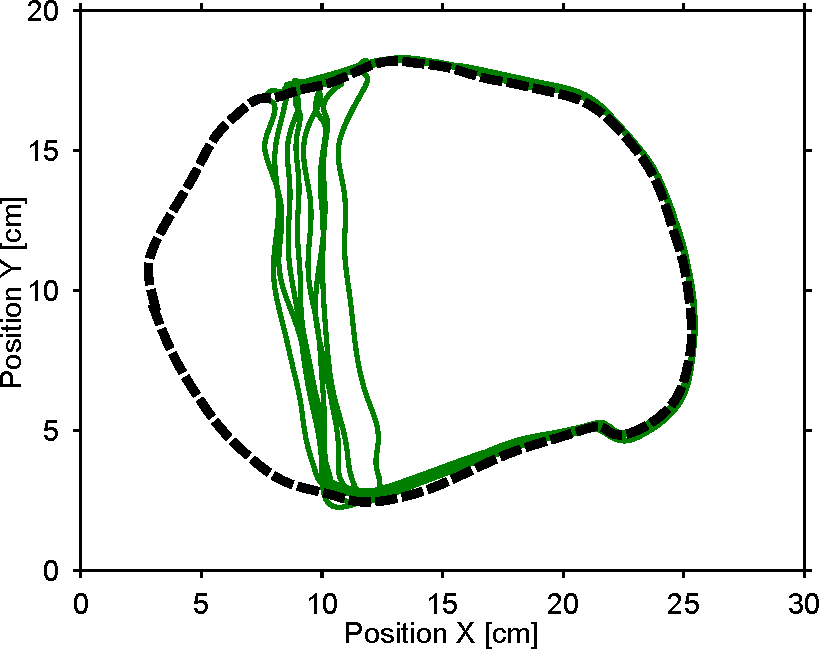
\includegraphics[width=.99\columnwidth]{robertoICRA/fig/Double_contact_b}
% 			\caption{Left contact}
% 			\label{fig:exp3:effects_contacts_pos:b}
% 		\end{subfigure}
% 		\hfill
% 		\begin{subfigure}[t]{0.32\hsize}
% 			\centering
% 			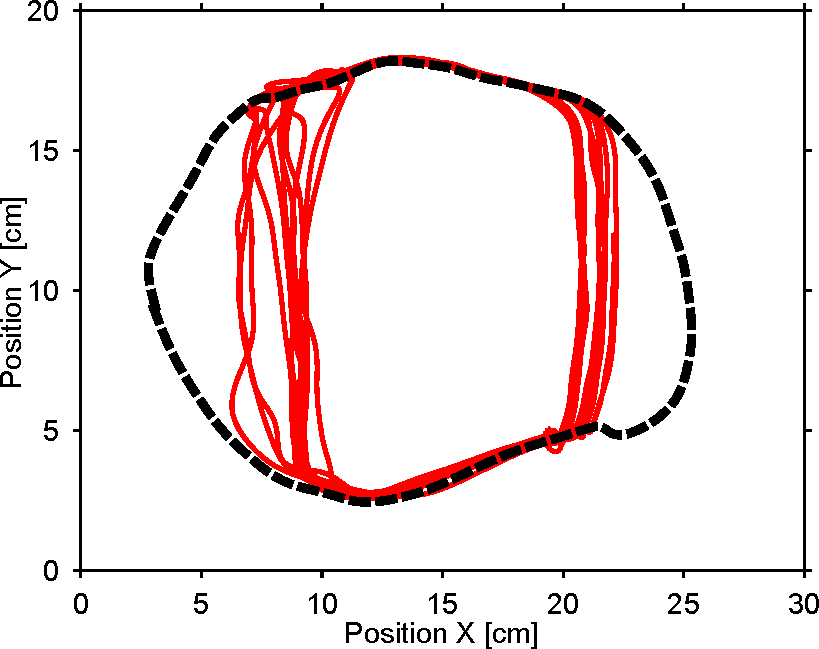
\includegraphics[width=.99\columnwidth]{robertoICRA/fig/Double_contact_c}
% 			\caption{Both contacts}
% 			\label{fig:exp3:effects_contacts_pos:c}
% 		\end{subfigure}
% 		\caption{\textbf{\nameref{sec:results:exp3}:} Effect of contacts in the task space for the three different case of contacts - \textcolor{blue}{right contact}, \textcolor{darkgreen}{left contact} and \textcolor{red}{both left and right contacts}. 
% 		The task in absence of contact is displayed as reference (\textbf{black dashed curve}). 
% 		%\comment{Figure generated by \textit{SomeFigures}}
% 		}
% 		\label{fig:exp3:effects_contacts_pos}
% 	\end{figure}
% 	%
 %

	%\begin{wrapfigure}{r}{0.46\columnwidth}
	\begin{figure}[t]
		\begin{minipage}{.32\linewidth}
			\centering
			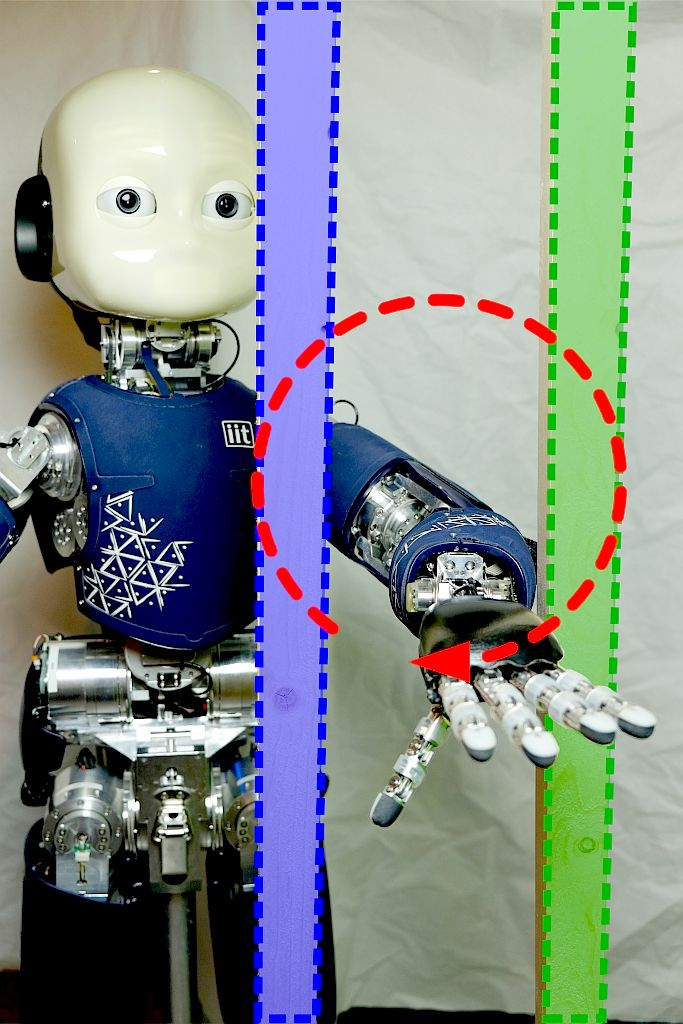
\includegraphics[width =.99\linewidth]{robertoICRA/fig/iCubParis02_Double_Contact}
			\caption{\textbf{\nameref{sec:results:exp3}:} The robot performs a circle with its left arm. 
			The forearm collides alternatively with the left, the right or both contacts.}
			\label{fig:exp3:icuparis_experiment_bars}
		\end{minipage}	
		\hfill
		\begin{minipage}{.52\linewidth}
			\centering
			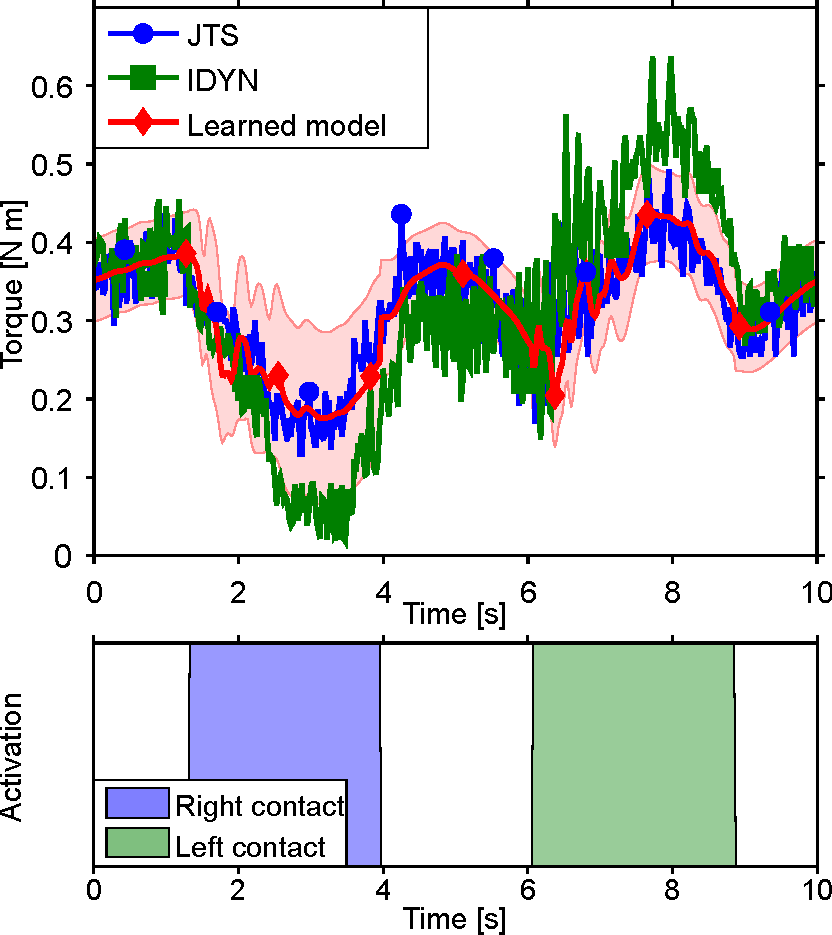
\includegraphics[width=.99\linewidth]{robertoICRA/fig/exp3_both}
			\caption{\textbf{\nameref{sec:results:exp3}:} Prediction of torques with multiple contacts and the corresponding activation of the gating network.
			%Various models are shown, but individually, none of them correctly capture the dynamics of the system. 
			Our mixture-of-experts model combines single-contact models to a multiple-contact model.
			}
			\label{fig:exp3:gating}
		\end{minipage}	
        \figspace
	\end{figure}
	%\end{wrapfigure}
	%


%===============================================================================

\subsection{Learning the gating network}
\label{sec:results:exp5}

	%An important component of our model is the gating network, which activates the different experts~$f_j$.
    %\todo[inline]{This is the first time I'm reading about experts...}
	So far, we assumed a heuristic gating network to select the active experts.
	%However, with growing complexity of the number and types of contacts, also the complexity of the gating network increases.
	%Hence, it will be valuable to automatically learn the gating network, which is equivalent to learning a classifier, which detects and recognizes the various types of contacts.
	In this experiment we show that a learned gating network achieves a comparable accuracy as a manually devised heuristic.
    As ground truth to evaluate the performances, as well as for training the classifier, we labeled the data with one of the following labels: no contact, left contact, right contact.
    The heuristic is based on thresholds of the activation of the skin input~$\skinInput$ and the force torque sensors~$\ftsForces$.
	We train a Support Vector Machine (SVM) classifier (using the library LIBSVM~\cite{Chang2011}) having as input $\q, \skinInput, \ftsForces$ and as output the contact labels (none, left, right).

	We evaluated the performance of the trained classifier on an unseen test set.
	\fig\ref{fig:exp5:accuracy} shows that the learned SVM achieved a classification accuracy that is similar to the heuristic gating network. 
    Equivalent results are obtained in terms of RMSE of the inverse dynamics when comparing the experts models learned by the gating networks.
    %A similar result is indicated in terms of RMSE when using the experts models based on the gating networks (see \tab\ref{tab:exp5b}).
    However, training the gating network (i.e., training the SVM classifier) requires considerably less expert knowledge compared to designing a heuristic. 
    As there is no visible performance difference, we conclude that training the gating network is generally preferable.
Increasing the number of training data may further increase the accuracy of the gating network.




% 	% 
% 	\begin{table}[t]
% 		\resizebox{\hsize}{!}{
% 		\centering
% 		\begin{tabular}{|l|c|c|c|}
% 			\hline 
% 			Gating network	& No Contact & Contact 1 & Contact 2 \\
% 			\hline 	
% 			Heuristic		&		\%	& x\% & x\% \\ 
%               Learned 		& 94.2 \%   		& 89.1 \% & 75.9 \% \\ 
% 			\hline
% 		\end{tabular}
% 		}
%  		\caption{\textbf{\nameref{sec:results:exp5}:} Classification accuracy for the heuristic gating network and the learned one using SVM.}
% 		\label{tab:exp5a}
% 	\end{table}
% 	%
% 	% 
% 	\begin{table}[t]
% 		\resizebox{\hsize}{!}{
% 		\centering
% 		\begin{tabular}{|l|c|c|c|}
% 			\hline 
% 			Gating network	& Shoulder 1 [Nm] & Shoulder 2 [Nm] & Elbow [Nm] \\
% 			\hline 	
% 			Learned (SVM)& $0.057 \pm 9.72\times 10^{-4}$ & $0.140 \pm 4.36\times 10^{-3}$ & $0.033 \pm 5.42\times 10^{-4}$\\ 
% 			Heuristic 		& $0.057  \pm 5.42\times 10^{-4}$ & $0.140  \pm 3.74\times 10^{-4}$ & $0.034 \pm 5.72\times 10^{-4}$\\ 
% 			\hline
% 		\end{tabular}
% 		}
% 		\caption{\textbf{\nameref{sec:results:exp5}:} Comparison of the RMSE when using the heuristic gating network and the learned one using SVM.}
% 		\label{tab:exp5b}
% 	\end{table}
% 	%